\documentclass[11pt,a4paper]{article}

\usepackage[T1]{fontenc}
\usepackage[scaled=1]{helvet}
\renewcommand{\familydefault}{\sfdefault}
\usepackage[margin=0.78in]{geometry}
\usepackage{setspace}
\setstretch{1.05}
\usepackage{graphicx}
\usepackage{booktabs}
\usepackage{float}
\usepackage[hidelinks]{hyperref}
\usepackage{enumitem}
\usepackage{tikz}
\usetikzlibrary{arrows.meta,positioning,fit,backgrounds}
\usepackage{titlesec}
\usepackage{amsmath}
\titleformat{\section}{\large\bfseries}{\thesection}{0.55em}{}
\titleformat{\subsection}{\normalsize\bfseries}{\thesubsection}{0.55em}{}
\titlespacing*{\section}{0pt}{8pt}{4pt}
\titlespacing*{\subsection}{0pt}{6pt}{3pt}
\setlist{nosep,leftmargin=*}
\setlength{\textfloatsep}{8pt}
\setlength{\intextsep}{7pt}

\newcommand{\ProjectTitle}{Auto Research for Materials Discovery}
\newcommand{\Programme}{AI6101}
\newcommand{\TeamMembers}{Qin Haochen, G2609647L}
\newcommand{\TODO}[1]{\textbf{TODO:} #1}

\begin{document}
\begin{center}
  {\LARGE\bfseries \ProjectTitle\par}
  \vspace{4pt}
\end{center}
\noindent\textbf{Course:} \Programme \hfill
\textbf{Team:} \TeamMembers\\
\textbf{Work type:} Individual project \hfill
\textbf{Code and results:} \texttt{autoresearch-for-materials-discovery}

\section*{Abstract}
I developed FARS (Feedback-Augmented Reinforcement Scheduler), a
Q-learning controller for MADE's ReAct materials-discovery agent. FARS
chooses between \textsc{Explore} and \textsc{Refine}; MADE's agent still
selects one structure for each official query. I also evaluated branch-search
state-Q, which uses RandomGenerator and ORB without LLM calls. Across five
60-query runs, branch-search had the highest mean observed-hull mSUN@60
(25.2) and AUDC (862.6) among the compared methods, including five-run
DeepSeek FARS (23.4; 744.1) and FARS-MQ (22.6; 688.1). This is an
exploratory result on one system, not evidence of more confirmed
ground-truth discoveries: branch-search had substantial run-to-run
variation and zero exact ground-truth formula or structure matches.

\section{Introduction}
Materials discovery is a sequential search: propose a structure, evaluate
it, then use the result to choose the next query. MADE provides a closed-loop
benchmark for this process \cite{made,repo}. My goal was to test whether a
small learned research scheduler could help allocate a fixed query budget.
This is an AI-systems project; I did not train a materials model.

\section{Method and Novelty}
My contribution is a bounded scheduler that adds online, feedback-driven
selection between MADE's existing generators without changing its
candidate evaluator or oracle. The novelty is this integration and its
evaluation in MADE's closed-loop setting, rather than a new reinforcement
learning algorithm or a new materials model.

I separately evaluated a state-conditioned branch-search controller. Unlike
FARS, this workflow uses MADE's RandomGenerator to propose a candidate slate,
selects the first candidate in that slate, and does not call an LLM. Its
branch/action Q-policy receives binary observed-discovery reward.

\paragraph{New code-only variant (not evaluated).}
I added a separate method named MADE-ReAct Branch Search. Its state-Q
controller still chooses the branch and action; MADE's planner and
RandomGenerator create that branch's slate, then MADE's
\texttt{LLMReActOrchestratorAgent} inspects and selects only from that slate
using selection tools. Candidate generation, branch constraints, oracle
evaluation, and the observed binary Q reward remain in the branch-search
workflow. This variant has not been run and is not included in the reported
results or averages.

\subsection{Pipeline diagrams}
Figures~\ref{fig:fars-pipeline} and
\ref{fig:made-react-branch-pipeline} show the two distinct control
pipelines. FARS uses a ReAct-style reasoning-and-action agent
\cite{react}, with its macro-action selected by a separate Q-learning
controller. MADE-ReAct Branch Search instead uses state-Q to choose a
branch and search action, then restricts MADE's ReAct agent to selecting
from the generated slate. Both feedback paths use straight line segments
and return observed outcomes to their respective controllers. Q-learning
follows the established tabular update \cite{watkins}. The new variant is
unrun; the branch-search results reported here are from the original
LLM-free method.

\begin{figure}[H]
\centering
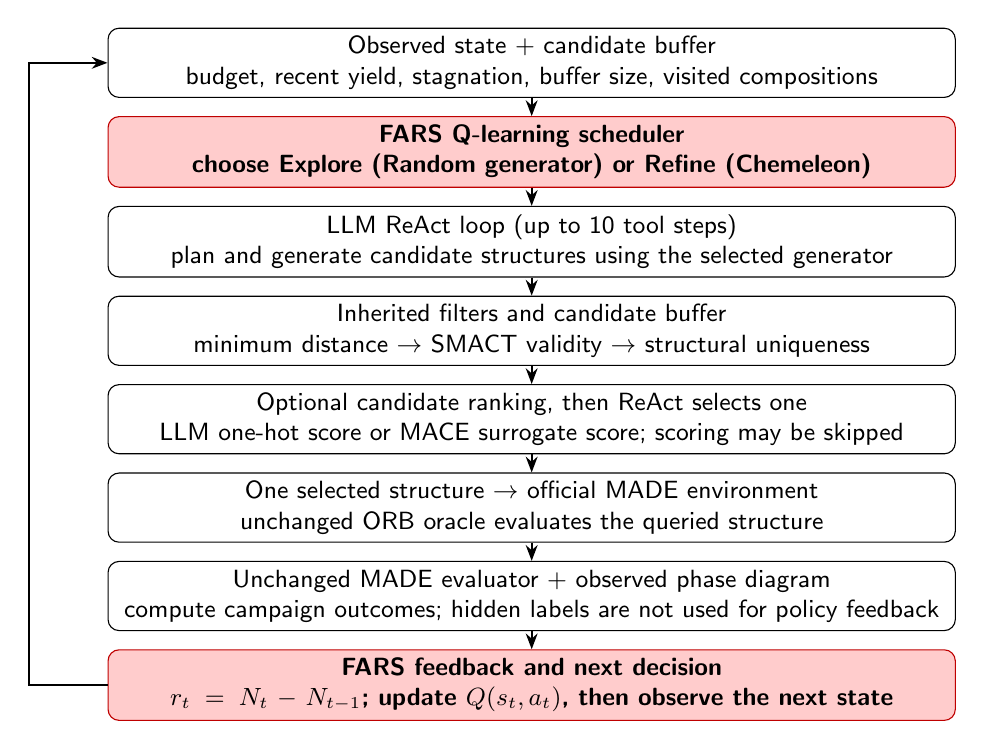
\begin{tikzpicture}[
  node distance=2.3mm,
  box/.style={draw,rounded corners,align=center,text width=0.87\linewidth,
    inner sep=3pt,font=\small},
  novel/.style={draw=red!75!black,fill=red!20,text=black,font=\small\bfseries},
  arr/.style={-{Stealth[length=2mm]},thick}
]
\node[box] (state) {Observed state + candidate buffer\\
  budget, recent yield, stagnation, buffer size, visited compositions};
\node[box,novel,below=of state] (scheduler) {FARS Q-learning scheduler\\
  choose \textsc{Explore} (Random generator) or \textsc{Refine} (Chemeleon)};
\node[box,below=of scheduler] (react) {LLM ReAct loop (up to 10 tool steps)\\
  plan and generate candidate structures using the selected generator};
\node[box,below=of react] (filters) {Inherited filters and candidate buffer\\
  minimum distance \(\rightarrow\) SMACT validity \(\rightarrow\) structural uniqueness};
\node[box,below=of filters] (scores) {Optional candidate ranking, then ReAct selects one\\
  LLM one-hot score or MACE surrogate score; scoring may be skipped};
\node[box,below=of scores] (query) {One selected structure \(\rightarrow\) official MADE environment\\
  unchanged ORB oracle evaluates the queried structure};
\node[box,below=of query] (eval) {Unchanged MADE evaluator + observed phase diagram\\
  compute campaign outcomes; hidden labels are not used for policy feedback};
\node[box,novel,below=of eval] (update) {FARS feedback and next decision\\
  \(r_t=N_t-N_{t-1}\); update \(Q(s_t,a_t)\), then observe the next state};
\draw[arr] (state) -- (scheduler);
\draw[arr] (scheduler) -- (react);
\draw[arr] (react) -- (filters);
\draw[arr] (filters) -- (scores);
\draw[arr] (scores) -- (query);
\draw[arr] (query) -- (eval);
\draw[arr] (eval) -- (update);
\draw[arr] (update.west) -- ++(-1.0,0) |- (state.west);
\end{tikzpicture}
\caption{FARS reuses MADE's pipeline. Optional LLM or MACE scoring ranks
candidates before selection; each selected structure is still evaluated by
the unchanged ORB oracle. The evaluator is unchanged.}
\label{fig:fars-pipeline}
\end{figure}

\begin{figure}[H]
\centering
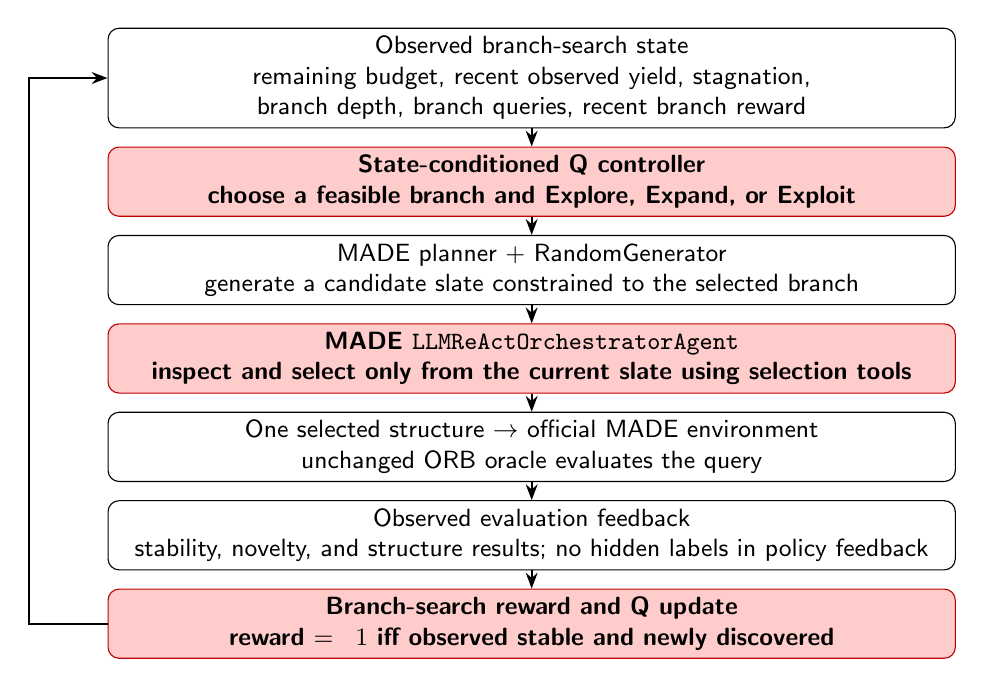
\begin{tikzpicture}[
  node distance=2.3mm,
  box/.style={draw,rounded corners,align=center,text width=0.87\linewidth,
    inner sep=3pt,font=\small},
  novel/.style={draw=red!75!black,fill=red!20,text=black,font=\small\bfseries},
  arr/.style={-{Stealth[length=2mm]},thick}
]
\node[box] (state) {Observed branch-search state\\
  remaining budget, recent observed yield, stagnation, branch depth,
  branch queries, recent branch reward};
\node[box,novel,below=of state] (controller) {State-conditioned Q controller\\
  choose a feasible branch and \textsc{Explore}, \textsc{Expand}, or \textsc{Exploit}};
\node[box,below=of controller] (slate) {MADE planner + RandomGenerator\\
  generate a candidate slate constrained to the selected branch};
\node[box,novel,below=of slate] (react) {MADE \texttt{LLMReActOrchestratorAgent}\\
  inspect and select only from the current slate using selection tools};
\node[box,below=of react] (query) {One selected structure \(\rightarrow\) official MADE environment\\
  unchanged ORB oracle evaluates the query};
\node[box,below=of query] (observe) {Observed evaluation feedback\\
  stability, novelty, and structure results; no hidden labels in policy feedback};
\node[box,novel,below=of observe] (update) {Branch-search reward and Q update\\
  reward \(=1\) iff observed stable and newly discovered};
\draw[arr] (state) -- (controller);
\draw[arr] (controller) -- (slate);
\draw[arr] (slate) -- (react);
\draw[arr] (react) -- (query);
\draw[arr] (query) -- (observe);
\draw[arr] (observe) -- (update);
\draw[arr] (update.west) -- ++(-1.0,0) |- (state.west);
\end{tikzpicture}
\caption{New, unrun MADE-ReAct Branch Search variant. The state-Q policy
chooses the branch and action; MADE generates the branch-constrained slate,
and its ReAct agent may select only from that slate. Red background with
bold black text marks the novel scheduler, ReAct selection, and feedback
components. The original branch-search results use the LLM-free
first-candidate selector, not this variant.}
\label{fig:made-react-branch-pipeline}
\end{figure}

\subsection{Actions, scores, and learning}
The scheduler state is a compact key made from budget remaining, recent
discovery yield, queries since discovery, candidate-buffer size, and visited
compositions. It chooses between feasible actions using epsilon-greedy
Q-learning. In the training runs, \(\epsilon=0.2\), learning rate
\(\alpha=0.2\), and discount \(\gamma=0.9\). Q-learning is a standard
temporal-difference update \cite{watkins}.

The Q-value scores a scheduler action, not a candidate. Let \(N_t\) be the
number of queried, newly discovered structures stable on the current
\emph{observed} hull. FARS uses the signed reward and standard Q-learning
update \cite{watkins}:
\begin{equation}
 r_t=N_t-N_{t-1}, \qquad
 Q(s_t,a_t)\leftarrow Q(s_t,a_t)+\alpha
 \left[r_t+\gamma\max_{a'}Q(s_{t+1},a')-Q(s_t,a_t)\right].
\end{equation}
The signed change can be negative if a later observed-hull update changes a
previous stability decision. The runner does not apply an online update
after the final query.

MADE also has optional candidate scorers. The LLM scorer assigns score
\(s_i=1\) to the candidate it selects and \(s_j=0\) to the other candidates.
The configured MACE surrogate scorer uses \(s_i=-E_{\mathrm{hull},i}\);
lower predicted distance above the \emph{observed} hull gives a higher score.
These scores only rank candidates; they are neither ORB labels nor FARS
Q-values. Scoring is optional and was not used for every proposal.

\subsection{FARS-MQ: supplied-Q initialization}
FARS-MQ is a warm-start configuration, not a different reward or
candidate-generation method. It loads a supplied table of 25 states and 50
state-action values, then uses the same features, actions, reward, and
online updates as fresh-start FARS. The initializer is read-only; each run
saves its own updated Q-table. Fresh-start FARS begins with an empty table.

The initializer is labelled a mean-Q table, but its source runs and
aggregation record were not supplied. I verified that it loaded, not that it
is an arithmetic mean. Lookup is exact: unfamiliar state keys receive no
transferred value. Across the original three FARS-MQ runs, 31 of 180
decisions (17.2\%) matched an initializer state, spanning 8 of 33 visited
states. This coverage does not show that initialization caused any
performance difference.

\begin{table}[H]
\centering
\small
\begin{tabular}{@{}rllrrlp{0.29\linewidth}@{}}
\toprule
Query & State key & Chosen & \(Q_E\) & \(Q_R\) & Reward & Interpretation\\
\midrule
4 & \texttt{3|high|recent|large|few} & REFINE & 0.000 & 0.200 & 0 & Higher Q; greedy-consistent\\
5 & \texttt{3|high|recent|large|few} & EXPLORE & 0.000 & 0.196 & 0 & Lower-Q choice; epsilon branch required\\
6 & \texttt{3|high|recent|large|few} & REFINE & 0.035 & 0.196 & 0 & Higher Q; greedy-consistent\\
\bottomrule
\end{tabular}
\caption{Examples from FARS seed 1. \(Q_E\) and \(Q_R\) are EXPLORE and
REFINE values at choice time. For query 5, EXPLORE has the lower Q-value, so
the epsilon-greedy policy requires the exploration branch.}
\label{tab:action}
\end{table}

\section{Evaluation}
All runs used a 60-query budget on the development system
\texttt{Cd-Li-Nd-Ti-W}, the official runner, ORB v3 with FIRE relaxation,
and a 0.1 eV/atom stability tolerance. The expanded comparison uses five
completed runs for branch-search, Random, Chemeleon, DeepSeek FARS, and
DeepSeek FARS-MQ. FARS with Qwen2.5-Coder 7B has three completed runs.
Several five-run groups combine the original seeds 1--3 with two additional
runs that reuse seed labels 1 and 2; they are five completed runs, not five
independent seeds. Custom LLM proposals were capped at 32 generated and 32
scored unique candidates per query, with a 1,920 generation cap. Random and
Chemeleon each generated a 1,024-candidate pool and queried one structure
at a time.

\noindent The primary metric, mSUN@60, is the final count of stable, unique,
novel discoveries. AUDC measures how quickly discoveries accumulate;
nAUDC divides it by the ideal 60-query area (1,800). Official AF/EF could
not be computed because the required baseline history was unavailable.
Table~\ref{tab:results} reports means and sample standard deviations across
the completed runs for each arm; it does not treat repeated seed labels as
independent random seeds. Random/Chemeleon, Qwen FARS, and DeepSeek FARS
are included as separate arms.
I report both the all-available-run means and the separate seeds-1--3
comparison: the former uses more completed campaigns, while the latter
avoids repeated seed labels. The five-run groups are descriptive campaign
aggregates, not five independent-seed replications.

\section{Results and Discussion}
\begin{table}[H]
\centering
\scriptsize
\resizebox{\linewidth}{!}{%
\begin{tabular}{@{}p{0.21\linewidth}p{0.19\linewidth}crrrr@{}}
\toprule
Method & LLM / proposer & \(n\) & mSUN@60 & AUDC & nAUDC & Valid\\
\midrule
Random generator & None & 5 & \(8.60\pm2.88\) & \(326.70\pm99.27\) & 0.1815 & 85.7\%\\
Chemeleon & None & 5 & \(8.80\pm2.86\) & \(280.20\pm98.55\) & 0.1557 & 99.3\%\\
FARS & Qwen2.5-Coder 7B & 3 & \(5.33\pm2.08\) & \(192.33\pm92.57\) & 0.1069 & 100.0\%\\
FARS & DeepSeek Flash & 5 & \(23.40\pm14.54\) & \(744.10\pm437.74\) & 0.4134 & 100.0\%\\
FARS-MQ & DeepSeek Flash & 5 & \(22.60\pm2.88\) & \(688.10\pm171.78\) & 0.3823 & 100.0\%\\
\textbf{Branch-search state-Q} & \textbf{None} & \textbf{5} & \(\mathbf{25.20\pm11.61}\) & \(\mathbf{862.60\pm372.86}\) & \textbf{0.4792} & 81.0\%\\
\bottomrule
\end{tabular}
}
\caption{Official discovery metrics across the completed 60-query runs.
mSUN@60 and AUDC are mean \(\pm\) sample SD. nAUDC is mean AUDC divided by
1,800; validity is the mean distance-and-SMACT valid fraction. The five-run
arms include repeated seed labels; FARS (Qwen) has three runs. Branch-search
and the two generator baselines make no LLM calls.}
\label{tab:results}
\end{table}

\begin{figure}[H]
\centering
\includegraphics[width=0.98\linewidth]{results/comparison-budget-60/cumulative-discovery-curve.png}
\caption{Mean observed-hull mSUN over 60 queries for six methods. Five runs
are shown for five arms; Qwen FARS has three completed runs. Several arms
reuse seed labels for repeated campaigns. Shading is \(\pm1\) sample SD, not
a confidence interval.}
\label{fig:curve}
\end{figure}

\begin{figure}[H]
\centering
\includegraphics[width=0.98\linewidth]{results/comparison-budget-60/cumulative-discovery-curve-three-distinct-seeds.png}
\caption{Like-for-like seed-count view using only original seeds 1--3 for all
six methods. Repeated campaigns are excluded. Shading is \(\pm1\) sample SD.}
\label{fig:three-seed-curve}
\end{figure}

Branch-search state-Q produced the highest mean observed-hull mSUN@60
(25.20) and mean AUDC (862.60) among these completed arms while using no
LLM calls. Its mean mSUN@60 was 1.80 above five-run DeepSeek FARS and 2.60
above five-run FARS-MQ, but the sample standard deviations are large and
overlapping; this descriptive comparison does not establish a statistically
reliable advantage. The branch-search workflow is also not a matched LLM
ablation: it uses the RandomGenerator, a different branch-based search
policy, and first-in-slate selection. All five branch-search runs had zero
exact ground-truth formula or structure matches. Therefore its larger mSUN
and AUDC reflect observed-hull stability discoveries, not verified
ground-truth material discoveries.

The no-repeat seed-1--3 view tempers this result: branch-search averaged
21.00 mSUN@60 (26, 17, 20), below FARS-MQ's 22.67 (20, 21, 27) and above
DeepSeek FARS's 18.67 (10, 13, 33). Thus, the five-run available comparison
shows a promising aggregate, not a consistent win across all run
selections.

Across the five available runs, FARS-MQ averaged 22.60 mSUN@60 and 688.10
AUDC; fresh-start DeepSeek FARS averaged 23.40 and 744.10. These overlapping
descriptive results do not show that the supplied initializer improves
performance. The two generator baselines averaged 8.60 (Random) and 8.80
(Chemeleon) mSUN@60; Qwen FARS averaged 5.33 across its three runs.

\subsection{Initializer coverage and candidate selection}
All three DeepSeek FARS-MQ runs loaded the same supplied initializer (25
states, 50 state-action values). Its contributing tables and aggregation
record are unavailable, so I verified that it loaded but not that it is an
arithmetic mean. Exact state-key matches occurred in 31 of 180 decisions
(17.2\%), spanning 8 of 33 visited states. Fresh-start FARS had 24 state
matches in 180 decisions; state overlap does not establish a benefit from
initialization.

Reduced formulas repeated after their first selection in 140/180 FARS-MQ
queries and 131/180 FARS queries, mostly during \textsc{Refine}. However,
all 360 queried structures had distinct MADE structure hashes. Thus,
repeated formulas were not exact structure duplicates, and these data alone
do not justify a formula-diversity constraint. Controller logs for these
runs contain no hidden-ground-truth reads. Detailed counts are in
\texttt{results/comparison-budget-60/candidate-selection-state-coverage.csv}.

\subsection{Observed outcomes and limitations}
In one Qwen FARS run, the selected formula was \texttt{Cd1} for 57/60
queries. Scheduler action values were tied on 52, 60, and 52 decisions
across the three runs. This indicates formula-level concentration and
weakly differentiated action values, not proven exploitation around known
successes. In one Random run, 51/60 candidates exceeded the stability
tolerance. These examples show how a fixed query budget can be spent on
concentrated or unstable proposals; neither is a general estimate from one
trajectory. FARS adapts only through online observed rewards and
epsilon-greedy action selection; it has no separate failure detector or
guaranteed strategy switch. I tested one composition system, did not use
the original GPT-5.1 configuration, and Chemeleon did not expose a
configured seed in this setup.

\section{Conclusion}
I implemented FARS as a bounded Q-learning scheduler around MADE's
unchanged ReAct agent and evaluation loop, and evaluated a separate
LLM-free branch-search state-Q method. Branch-search had the highest
observed-hull mean mSUN@60 and AUDC in the completed comparison, despite
making no LLM calls. However, the five-run sample is variable, its runs had
zero exact ground-truth matches, and the compared search workflows were not
matched. The result supports branch-search as a promising low-LLM-cost
direction, not a confirmed claim of better material discovery. One system,
repeated seed labels in several groups, and unverified FARS-MQ initializer
provenance limit generalization and causal interpretation.

\subsection{Future work}
I will first obtain the initializer's source tables and aggregation record,
then run a paired fresh-start versus initialized comparison using
predeclared, unique seeds and otherwise matched settings. I will also test
candidate limits (32, 64, and 128) one factor at a time.

\appendix
\section{Supplementary comparisons}
\label{app:supplementary}

\subsection{Run counts and reproducibility}
Five completed runs are available for Random, Chemeleon, DeepSeek FARS,
DeepSeek FARS-MQ, and branch-search state-Q; Qwen FARS has three. Random,
Chemeleon, and both DeepSeek FARS arms combine the original three runs with
two repeat campaigns using reused seed labels 1 and 2. Branch-search uses
five distinct seeds. Figure~\ref{fig:three-seed-curve} excludes repeat
campaigns and shows original seeds 1--3 for all six arms. The per-run source
metrics and both discovery-curve datasets are recorded in
\texttt{results/comparison-budget-60/six-methods-run-metrics.csv},
\texttt{six-methods-summary-metrics.csv}, and
\texttt{six-methods-discovery-curves.csv}; the original-seed summary is in
\texttt{six-methods-three-distinct-seed-summary.csv}.

\subsection{Branch-search state-Q}
I also completed five 60-query branch-search runs on
\texttt{Cd-Li-Nd-Ti-W}, using seeds 1--5. This method uses a tabular
state-Q controller to select branches in a search tree; candidates are
proposed by MADE's RandomGenerator and evaluated by the ORB oracle. It uses
no LLM, unlike FARS and FARS-MQ, and is a distinct search workflow.

\begin{table}[H]
\centering
\small
\begin{tabular}{@{}crr@{}}
\toprule
Seed & mSUN@60 & Official AUDC\\
\midrule
1 & 26 & 764.0\\
2 & 17 & 468.5\\
3 & 20 & 636.0\\
4 & 45 & 1,423.5\\
5 & 18 & 1,021.0\\
\midrule
Mean \(\pm\) sample SD & \(25.20\pm11.61\) & \(862.60\pm372.86\)\\
\bottomrule
\end{tabular}
\caption{Branch-search state-Q outcomes across five completed 60-query runs.
mSUN is the number stable on the observed hull, not the number confirmed
against hidden ground truth.}
\label{tab:branch-search-results}
\end{table}

The branch-search runs reported zero exact ground-truth formula or structure
matches. Their mSUN counts therefore describe observed-hull discoveries,
not verified ground-truth hits. The FARS and new MADE-ReAct Branch Search
feedback loops are shown separately in Figures~\ref{fig:fars-pipeline} and
\ref{fig:made-react-branch-pipeline}. The five branch-search runs reported
above used the original LLM-free variant.

\clearpage
\section*{References}
\begin{thebibliography}{9}
\setlength{\itemsep}{2pt}
\bibitem{made}
S. A. Malik, T. Doherty, P. Tigas, M. Razzak, S. J. Roberts, A. Walsh, and
Y. Gal, ``MADE: Benchmark Environments for Closed-Loop Materials Discovery,''
arXiv:2601.20996v2, 2026.
\bibitem{react}
S. Yao et al., ``ReAct: Synergizing Reasoning and Acting in Language Models,''
in \emph{International Conference on Learning Representations}, 2023.
\bibitem{watkins}
C. J. C. H. Watkins and P. Dayan, ``Q-learning,''
\emph{Machine Learning}, vol. 8, pp. 279--292, 1992.
\url{https://doi.org/10.1007/BF00992698}.
\bibitem{repo}
Diffractive Labs, ``MADE: MAterials Discovery Environments,'' source
repository and benchmark implementation.
\url{https://github.com/diffractivelabs/MADE}.
\end{thebibliography}
\end{document}
